\subsection*{A. Azat and bookshelf}
 

Азат готовится к сессии. Именно поэтому ему лезут в голову вопросы, которые мало относятся к подготовке к зачетам. Например, сколько надо деревянных опилок, чтобы сделать книжную полку, которая наполнилась знаниями в виде конспектов за целый семестр? Книжная полка  представляет собой прямоугольный параллелепипед без передней стенки. Все 5 стенок сделаны из фанеры толщиной $D$. А размеры полки по внешней стороне равны: $H$ (высота), $W$ (ширина) и  $L$ (глубина). Чтобы Азат мог приступить к изучению содержимого этой полки, помогите ему ответить на вопрос, какой объем фанерного листа был использован?

\begin{center}
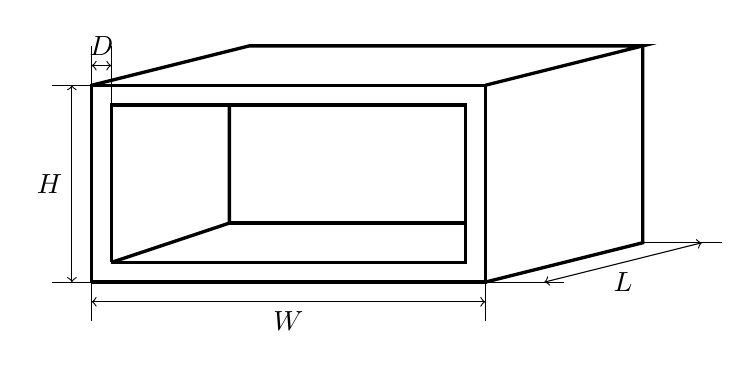
\begin{tikzpicture}[scale=0.25]
\draw[very thick] (0, 0) -- (20, 0) -- (20, 10) -- (0, 10) -- (0, 0);
\draw[very thick] (0, 10) -- (8, 12) -- (28, 12) -- (20, 10);
\draw[very thick] (28, 12) -- (28, 2) -- (20, 0);
\draw[very thick] (1, 1) -- (1, 9) -- (19, 9) -- (19, 1) -- (1, 1);
\draw[very thick] (1, 1) -- (7, 3) -- (7, 9);
\draw[very thick] (7, 3) -- (19, 3);
\draw[<->] (0, -1) -- node[below] {$W$} ++ (20, 0);
\draw[<->] (-1, 0) -- node[left] {$H$} ++ (0, 10);
\draw[<->] (23, 0) -- node[below] {$L$} ++ (8, 2);
\draw[<->] (0, 11) -- node[above] {$D$} ++ (1, 0);
\draw (20, 0) -- (24, 0);
\draw (28, 2) -- (32, 2);
\draw (20, -2) -- (20, 0);
\draw (0, 0) -- (0, -2);
\draw (-2, 0) -- (0, 0);
\draw (-2, 10) -- (0, 10);
\draw (0, 10) -- (0, 12);
\draw (1, 9) -- (1, 12);
\end{tikzpicture}
\end{center}

\informat{Четыре целых положительных числа $D$, $H$, $W$, $L$ от 1 до 1000, причем $2 D < \min(W, H, L)$.}

\outformat{Одно целое число --- объем листа.}

\examplee{1 3 3 3}{25}{1 10 20 30}{1824}

\subsection*{B. Bekarys and khet}

Бекарыс, вдохновленный лазерными шахматами khet, решил собрать собственную настольную игру. Игра проходит на поле размером $N \times M$ единичных клеток. Свет лазера попадает на доску через середину левой стороны левой верхней клетки. В некоторые клетки установлены двусторонние зеркала. Они расположены вдоль одной из диагоналей клетки. Количество очков равно общей длине лазерного пучка, который находится над игровыми полем. Помогите Бекарысу посчитать количество очков в текущей позиции.

\begin{center}
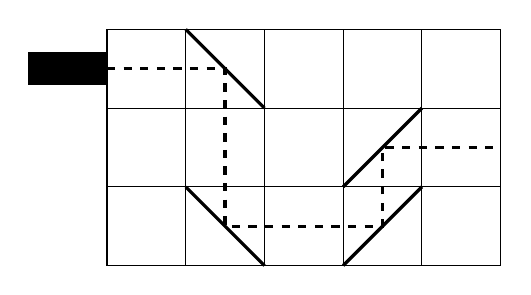
\begin{tikzpicture}
\draw[fill] (0,2.3) rectangle (-1.0, 2.7);
\draw (0,0) grid (5, 3);
\draw[very thick] (1, 3) -- (2, 2);
\draw[very thick] (1, 1) -- (2, 0);
\draw[very thick] (4, 1) -- (3, 0);
\draw[very thick] (4, 2) -- (3, 1);
\draw[dashed, very thick] (0, 2.5) -- (1.5, 2.5) -- (1.5, 0.5) -- (3.5, 0.5) -- (3.5, 1.5) -- (5.0, 1.5);
\end{tikzpicture}
\end{center}

\informat{В первой строке два целых числа $N$ и $M$ от 1 до 100 --- ширина и высота поля соответственно.
Далее $N$ строк (каждая длины $M$), которые описывают поле:\\
{\tt *} --- пустое поле;\\
{\tt /} --- зеркало из левого нижнего в правый верхний угол квадрата;\\
{\tt \textbackslash} --- зеркало из правого нижнего в левый верхний угол квадрата. \\ \mbox{}
}

\outformat{Одно целое число --- длина пути, который пройдет луч.}

\examplee
{
3 5 \newline
*\textbackslash***\newline
***/*\newline
*\textbackslash*/*
}
{8}
{
2 2 \newline
/\textbackslash \newline
\textbackslash/}
{1}




\subsection*{C. Computer vision}
 

Ануар занялся задачами компьютерного зрения. Он уже написал программу, которая распознает числа. Если программа не может достоверно определить цифру, она заменяет ее на звездочку. Ануар получил очередной результат своей программы в виде строки из звездочек и цифр. 

Ануару нравятся числа, которые делятся на 11. Поэтому он задумался, сколько различных чисел кратных 11 соответствуют такой строке? При этом Ануара абсолютно не смущают ведущие нули.

\informat{Строка длиной не более 100 000, содержащая символы цифр и звездочки.}

\outformat{Одно целое число --- количество подходящих чисел. Так как ответ может быть очень большим вывести его по модулю $10^9+7$.}

\exampleee{**}{10}{10*}{0}{1*1*}{9}




\subsection*{D. DPK rover}
 

Димитрий, Павел и Куат управляют группой марсоходов с секретным названием DPK. Все марсоходы изначально находятся на базе, где хранится неограниченный запас топлива. Полный бак топлива позволяет проехать марсоходу расстояние $D$. При движении марсоход расходует топливо пропорционально пройденному расстоянию, а пока стоит на месте, не расходует топлива вовсе. Любой марсоход может отдать любую часть топлива другому марсоходу с учетом ограниченности бака.

Ребята хотят отвезти флаг базы как можно дальше согласно хитрому плану. Одновременно с базы выезжают все $M$ марсоходов. Через некоторое время все они разбиваются на \textbf{равные} группы. Из каждой группы ровно один марсоход продолжает путь, а остальные марсоходы из этой группы отдают ему топливо и возвращаются назад для дозаправки на базе или для дозаправки от других марсоходов. Далее оставшиеся марсоходы снова делятся на равные группы, пока не останется один марсоход, который и водрузит флаг. На какое максимальное расстояние марсоходы смогут увезти флаг от базы так, чтобы все смогли вернуться на базу?

\informat{Два целых числа $D$ (от 1 до 10) и $M$ (от 1 до $10^{12}$).}

\outformat{Одно вещественное число --- максимальное расстояние с точностью 5 знаков после запятой.}

\examplee{5 1}{2.500000}{6 2}{5.000000}

\excomm{Второй пример. Оба марсохода продвигаются на расстояние 2. Потом первый марсоход отдает второму половину оставшегося топлива, а сам возвращается на базу. Второй марсоход проезжает еще расстояние 3 и ставит флаг на отсечке в 5. После разворота он возвращается на расстояние 2, где его снова заправляет первый марсоход, который опять вернулся с базы. Для лучшего понимания смотрите схему.}

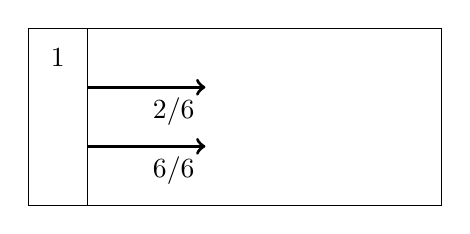
\begin{tikzpicture}[scale=0.75]
\draw (-1, -1) rectangle (6, 2);
\node at (-0.5, 1.5) {$1$};
\draw (0,-1) -- (0,2);
\draw[very thick, ->] (0, 1) -- (2, 1) node[below left] {$2/6$};
\draw[very thick, ->] (0, 0) -- (2, 0) node[below left] {$6/6$};
\end{tikzpicture}
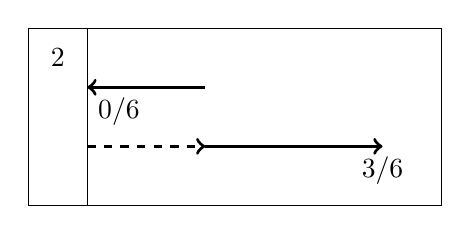
\begin{tikzpicture}[scale=0.75]
\draw (-1, -1) rectangle (6, 2);
\node at (-0.5, 1.5) {$2$};
\draw (0,-1) -- (0,2);
\draw[very thick, ->] (2, 1) -- (0, 1) node[below right] {$0/6$};
\draw[dashed, very thick, ->] (0, 0) -- (2, 0);
\draw[very thick, ->] (2, 0) -- (5, 0) node[below] {$3/6$};
\end{tikzpicture}

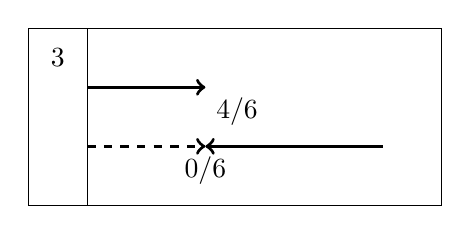
\begin{tikzpicture}[scale=0.75]
\draw (-1, -1) rectangle (6, 2);
\node at (-0.5, 1.5) {$3$};
\draw (0,-1) -- (0,2);
\draw[very thick, ->] (0, 1) -- (2, 1) node[below right] {$4/6$};
\draw[dashed, very thick, ->] (0, 0) -- (2, 0);
\draw[very thick, ->] (5, 0) -- (2, 0) node[below] {$0/6$};
\end{tikzpicture}
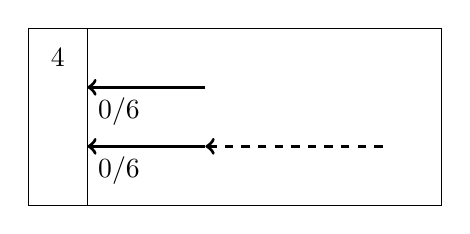
\begin{tikzpicture}[scale=0.75]
\draw (-1, -1) rectangle (6, 2);
\node at (-0.5, 1.5) {$4$};
\draw (0,-1) -- (0,2);
\draw[very thick, ->] (2, 1) -- (0, 1) node[below right] {$0/6$};
\draw[dashed, very thick, ->] (5, 0) -- (2, 0);
\draw[very thick, ->] (2, 0) -- (0, 0) node[below right] {$0/6$};
\end{tikzpicture}



\subsection*{E. Excellent idea}
 


Иногда всё хочется поставить с ног на голову. Например, поменять задания и вердикты местами! Данная предыстория не сильно помогает решить эту задачу. В отличии от Надиры и других выпускников, которые сильно помогают в проведении этой олимпиады!

\informat{Строка.}

\examplEEE{Memory limit exceeded, test 2}{e}{Presentation error, test 3}{e}{Time limit exceeded, test 4}{e}




\subsection*{F. Forced reduction}
 

Тимур любит изучать сложные структуры данных. Ерулан любит изучать простые структуры данных. Тимур зачем-то недавно рассказал про структуру данных <<бор>> Ерулану: <<бор --- это корневое дерево, каждое ребро которого помечено каким-то символом так, что для любого узла все рёбра, соединяющие этот узел с сыновьями, помечены разными символами.>>

Ерулан решил, что определение слишком сложное и надо бы его сократить. Полученную структуру он назвал <<недобор>>. А именно, <<недобор>> --- это корневое дерево, каждое ребро которого помечено каким-то символом.

Вершины дерева пронумерованы целыми числами от 1 до N, при этом 1 является корнем дерева. Как же найти в <<недоборе>> количество различных слов, которые можно получить, двигаясь по ребрам от корня? 

\informat{На первой строке целое число $N$ от 1 до $10^5$. Далее (N-1) строка. На $i$-й строке указан $p_i$ --- родитель $i$-й вершины и буква, соответствующая ребру между вершинами $p_i$ и $i$.}


\outformat{Одно целое число --- количество различных слов.}

\examplepic{
8 \newline
1 a \newline
5 d \newline
5 b \newline
1 a \newline
2 b \newline
6 c \newline
4 e
}{5}{Слова: a, ab, ad, abc, abe. \newline 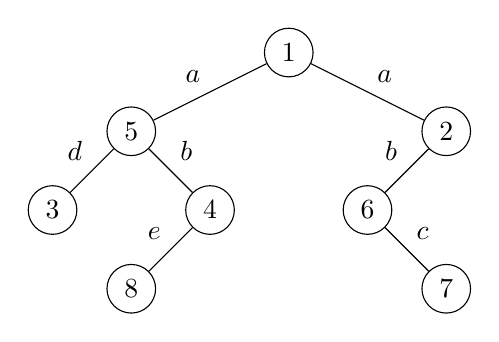
\begin{tikzpicture}

\node[circle, draw=black] (1) at (5, 5) {1};
\node[circle, draw=black] (5) at (3, 4) {5};
\node[circle, draw=black] (2) at (7, 4) {2};
\node[circle, draw=black] (3) at (2, 3) {3};
\node[circle, draw=black] (4) at (4, 3) {4};
\node[circle, draw=black] (6) at (6, 3) {6};
\node[circle, draw=black] (8) at (3, 2) {8};
\node[circle, draw=black] (7) at (7, 2) {7};

\draw (1) -- (2) node[midway, above right] {$a$};
\draw (2) -- (6) node[midway, above left] {$b$};
\draw (6) -- (7) node[midway, above right] {$c$};
\draw (1) -- (5) node[midway, above left] {$a$};
\draw (5) -- (4) node[midway, above right] {$b$};
\draw (4) -- (8) node[midway, above left] {$e$};
\draw (5) -- (3) node[midway, above left] {$d$};
%1-a-2-b-6-c-7
%|
%a
%|
%5-b-4-e-8
%|
%d
%|
%3

\end{tikzpicture}
}





\subsection*{G. Giant chandelier}
 

Чингиз, Вова и Агаси наслаждаются всеми прелестями проживания в общежитии. Для создания студенческого уюта они решили повесить в комнату люстру. Ребята выбрали гигантскую люстру-ежик с $N$ лампочками. Пытаясь определить, поместится ли люстра в комнате, Агаси начал крутить ее в руках. Но его роста оказалось не достаточно, чтобы подвесить люстру за соответствующее крепление. Поэтому он взял в руки эту люстру и попросил Вову и Чингиза зафиксировать положение всех лампочек в Агаси-центрированной прямоугольной системе координат. В этой системе крепление имеет координаты $(0, 0, 0)$, а $i$-я лампочка находится в точке $(x_i, y_i, z_i)$. Какой минимальной высоты должна быть комната, чтобы люстра целиком поместилась в комнату в подвешенном состоянии за крепление, после того как она развернется под действием силы тяжести?

Сила тяжести направлена вниз (вдоль вектора $(0, 0, -1)$). Все конструкции люстры, кроме лампочек, невесомы и жестко фиксированы друг относительно друга. Точка крепления не обязательно должна быть на потолке. Все лампочки имеют одинаковый вес и их можно считать точками. 

\informat{Одно целое число $N$ от 1 до $10^5$. Далее $N$ строк. В каждой по три целых числа $x_i$, $y_i$, $z_i$ от $-1000$ до $1000$. Гарантируется, что центр тяжести точек отличен от (0, 0, 0).}

\outformat{Одно вещественное число --- минимальная высота комнаты с точностью 5 знаков после запятой.}

\exampleee{
2 \newline
3 4 0 \newline
4 -3 0
}
{3.5355339}
{3 \newline
39 0 0 \newline
0 52 0 \newline
0 0 156
}
{144.0000000}
{2 \newline
1 0 0 \newline
-2 0 0
}
{3.0000000}

\excomm{В первом примере Агаси держит плоскую люстру горизонтально. Под действием силы тяжести люстра опустится вниз так, что координаты лампочек будут равны $\left(\frac{5 \sqrt{2}}{2}, 0, -\frac{5 \sqrt{2}}{2} \right)$ и $\left(-\frac{5 \sqrt{2}}{2}, 0, -\frac{5 \sqrt{2}}{2} \right)$ с точностью до поворота вокруг оси $OZ$. То есть достаточно высоты $\frac{5 \sqrt{2}}{2}$.}

\begin{center}
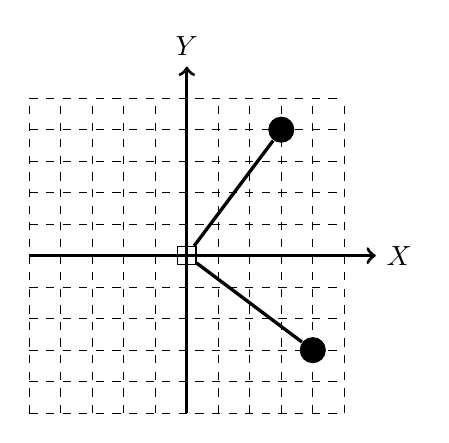
\begin{tikzpicture}[scale=0.4]

\draw[dashed] (-5, -5) grid (5, 5);

\draw[very thick, ->] (-5, 0) -- (6, 0) node[right]{$X$};
\draw[very thick, ->] (0, -5) -- (0, 6) node[above]{$Y$};

\node[circle, fill=black] (1) at (3, 4) {};
\node[circle, fill=black] (2) at (4, -3) {};
\node[rectangle, draw=black] (0) at (0, 0) {};

\draw[very thick] (0) -- (1);
\draw[very thick] (0) -- (2);

\end{tikzpicture}
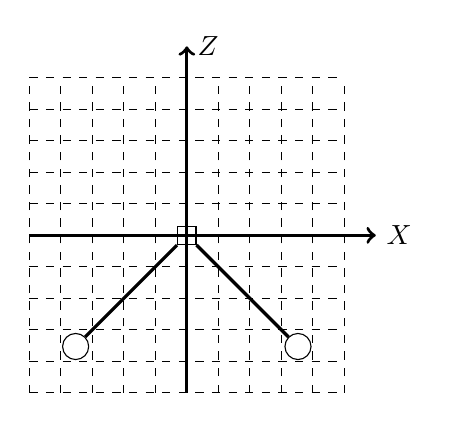
\begin{tikzpicture}[scale=0.4]

\draw[dashed] (-5, -5) grid (5, 5);

\draw[very thick, ->] (-5, 0) -- (6, 0) node[right]{$X$};
\draw[very thick, ->] (0, -5) -- (0, 6) node[right]{$Z$};

\node[rectangle, draw=black] (0) at (0, 0) {};
\node[circle, draw=black] (3) at (3.53, -3.53) {};
\node[circle, draw=black] (4) at (-3.53, -3.53) {};

\draw[very thick] (0) -- (3);
\draw[very thick] (0) -- (4);

\end{tikzpicture}
\end{center}





\subsection*{H. Hyper numbers}
 

Рамазан всё еще находится под впечатлением от теории чисел, которую сдал больше года назад. Иногда он придумывает свойства для чисел и дает таким числам интересные названия. К примеру, вот определение гипер-числа: $N$ --- является гипер-числом, если $D(N)$ содержит нечетное количество элементов, где $D(N)$ --- это множество чисел $X$ от 1 до $(N-1)$ таких, что $X$ и $N$ взаимно просты. Рамазан придумал очень хитрый способ находить количество всех гипер-чисел из заданного диапазона. А Вы сможете найти?

\informat{Два целых положительных числа $L$ и $R$ от 2 до $10^{18}$ и $L \leqslant R$.}

\outformat{Одно целое число --- количество гипер-чисел. Так как ответ может быть очень большим выведите ответ по модулю $10^9+7$.}

\example{2 3}{1}